
\documentclass[../open-optimization/open-optimization.tex]{subfiles}

\begin{document}


\url{https://www.youtube.com/watch?v=YX40hbAHx3s}

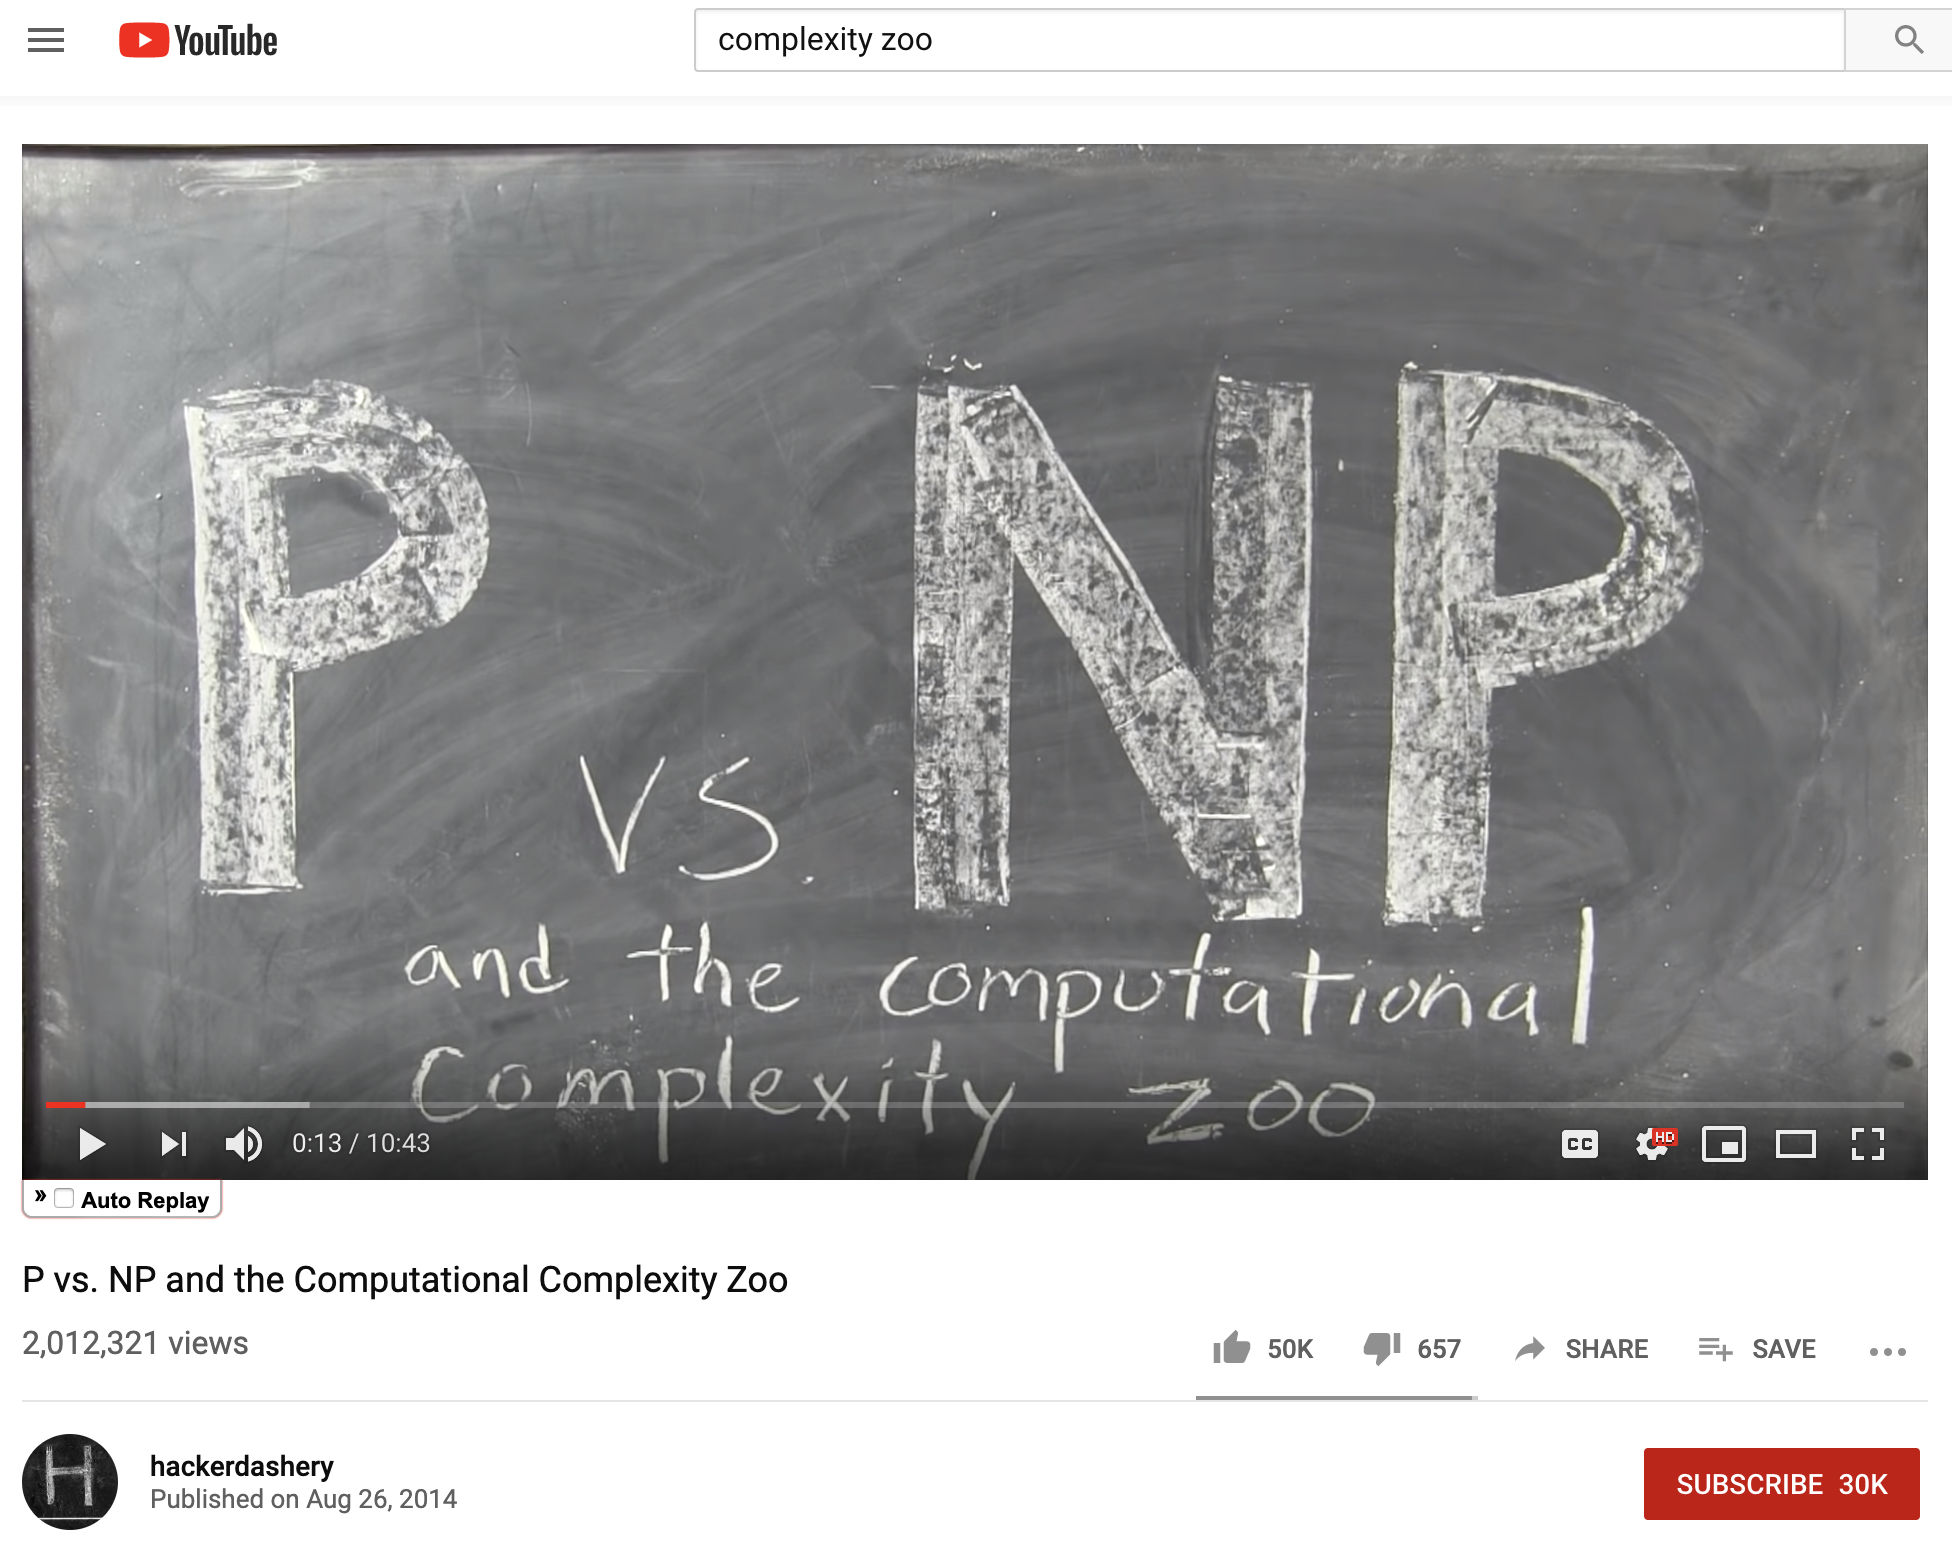
\includegraphics[scale = 0.15]{youtube-PvsNP}

When considering a problem class, we want to know roughly how difficult the problem is.  
When considering an algorithm, we want to know roughly how fast the algorithm will run.
These are questions that we can answer with complexity theory.

Binary:
\url{http://www.texample.net/tikz/examples/complement/}


%\includegraphics[scale = 0.5]{enigma}
%
%\includegraphics[scale = 0.5]{enigma-break}
%
%\url{https://en.wikipedia.org/wiki/Alan_Turing}

\section{Big-O Notation}

\begin{definition}[Big-O]
For two functions $f(n)$ and $g(n)$, we say that $f(n) = O(g(n))$ if there exist positive constants $c$ and $n_0$ such that 
\begin{equation}
\label{eq:bigO}
0 \leq f(n) \leq c\, g(n) \ \ \text{ for all } \ \ \ n \geq n_0.
\end{equation}
\end{definition}

\begin{center}
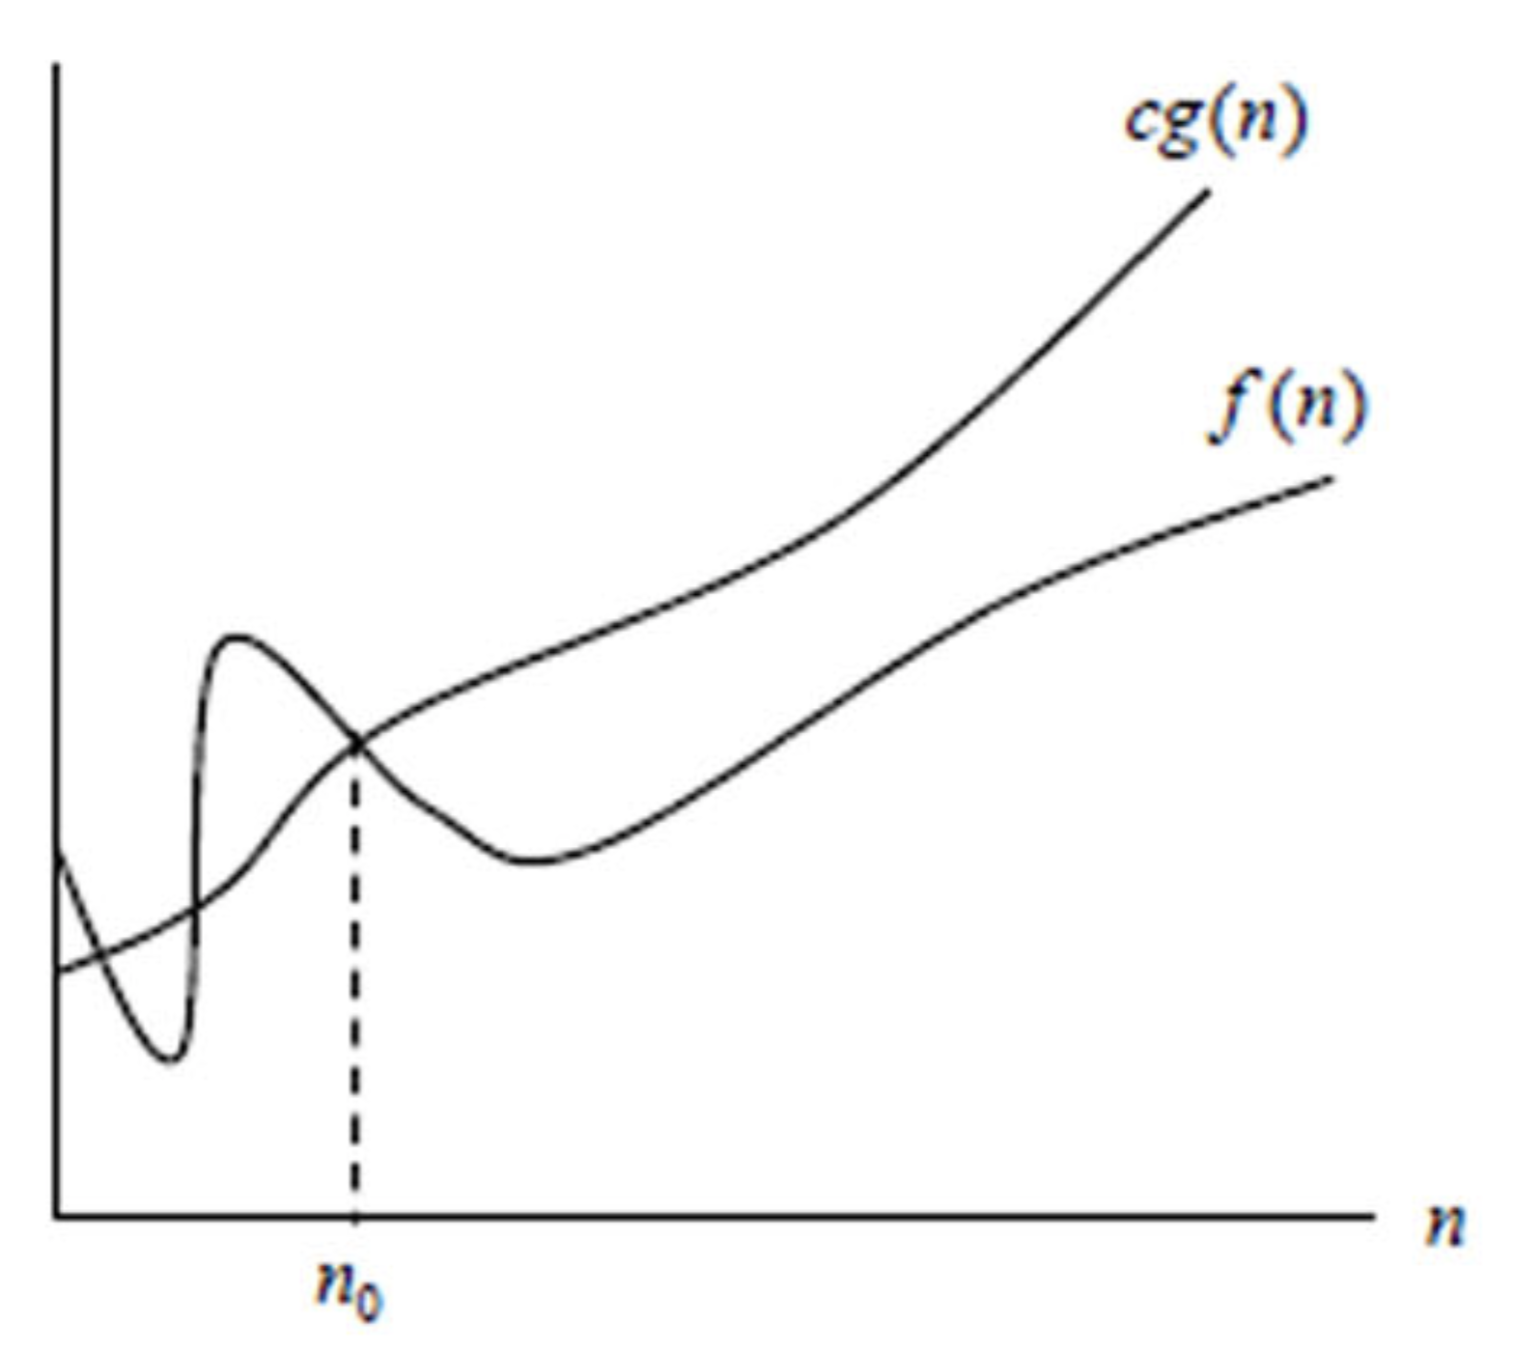
\includegraphics[scale = 0.15]{big-O}
\end{center}
\begin{figure}[H]
\begin{center}
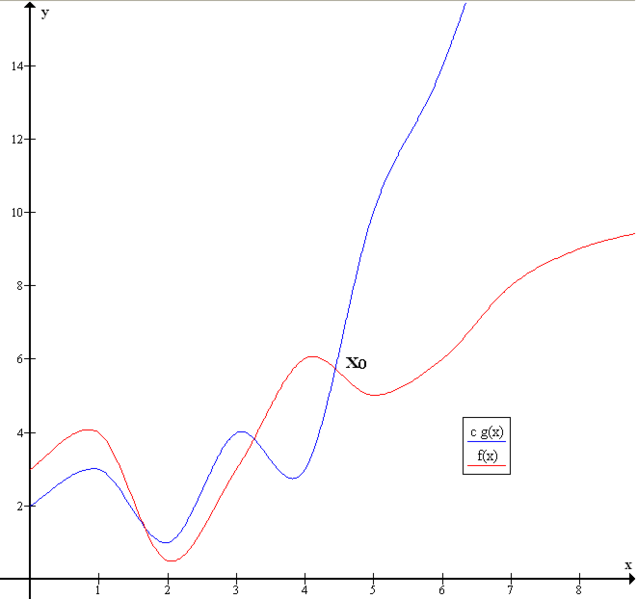
\includegraphics[scale = 0.15]{Big-O-notation}\footnotemark
\end{center}
\caption{Example of Big O notation: $f(x) \in O(g(x))$ as there exists $c > 0 $ (e.g. $c = 1$) and $x_0$ (e.g. $x_0 = 5$) such that $f(x) \leq cg(x)$ whenever $x \geq x_0$.}
\end{figure}
\footnotetext{Image borrowed from \url{https://commons.wikimedia.org/wiki/File:Big-O-notation.png}}
We can also use Big-O to denote a set as
\begin{multline}
O(g(n)) := \{ f(n) :\text{ there exist positive constants $c$ and $n_0$ such that}\\ \text{$0 \leq f(n) \leq c\,g(n)$, for all $n \geq n_0$}\}.
\end{multline}
\begin{example}
\label{ex:bigO}
Consider $f(n) = 5 n^2 + 10n + 7$ and $g(n) = n^2$.  We want to show that $f(n) = O(g(n))$.  

Let's try $c = 22$ and $n_0 = 1$.  We need to show that \autoref{eq:bigO} is satisfied.

Note first that we always have
\begin{enumerate}
\item $n^2 \leq n^2 \ \ \text{ and therefore } \ \ 5n^2 \leq 5n^2$
\end{enumerate}
Note that if $n \geq 1$, then 
\begin{enumerate}
\setcounter{enumi}{1}
\item $n \leq n^2 \ \ \text{ and therefore } \ \ 10n \leq 10 n^2$
\item $1 \leq n^2 \ \ \text{ and therefore } \ \  7 \leq 7 n^2$
\end{enumerate}
Since all inequalities 1,2, and 3 are valid for $n\geq 1$, by adding them, we obtain a new inequality that is also valid for $n \geq 1$, which is
\begin{align}
5n^2 + 10n + 7 &\leq 5n^2 + 10n^2 + 7 n^2 & \text{ for all } n \geq 1,\\
\Rightarrow \ \ \ \  5n^2 + 10n + 7  & \leq 22 n^2 & \text{ for all } n \geq 1.
\end{align}
Hence, we have shown that \autoref{eq:bigO} holds for $c = 22$ and $n_0 = 1$.  Hence $f(n) = O(g(n))$.
\end{example}



Correct uses:
\begin{itemize}
\item $2^n + n^5 + \sin(n) = O(2^n)$
\item $2^n = O(n!)$
\item $n! + 2^n + 5n = O(n!)$
\item $n^2 + n = O(n^3)$
\item $n^2 + n = O(n^2)$
\item $\log(n) = O(n)$
\item $10 \log(n) + 5 = O(n)$
\end{itemize}
Notice that not all examples above give a tight bound on the asymptotic growth.  For instance, $n^2 + n = O(n^3)$ is true, but a tighter bound is $n^2 + n = O(n^2)$.  

In particular, the goal of big O notation is to give an upper bound on the asymptotic growth of a function.  
But we would prefer to give a strong upper bound as opposed to a weak upper bound.
For instance, if you order a package online, you will typically be given a bound on the latest date that it will arrive.  For example, if it will arrive within a week, you might be guaranteed that it will arrive by next Tuesday.  This sounds like a reasonable bound.  But if instead, they tell you it will arrive before 1 year from today, this may not be as useful information.
In the case of big O notation, we would like to give a least upper bound that most simply describes the growth behavior of the function.

In that example,  
$n^2 + n = O(n^2)$, this literally means that 
there is some number $c$ and some value $n_0$ that 
$n^2 + n \leq c n^2$ for all $n \geq n_0$, 
that is, for all values of $n_0$ larger than $n$, the function $c n^2$ dominates $n^2 + n$.  

For example, a valid choice is $c = 2$ and $n_0 = 1$.  Then it is true that 
$n^2 + n \leq 2 n^2$ for all $n \geq 1$.



But it is also true that $n^2 + n = O(n^3)$.  For example, a valid choice is again $c = 2$ and $n_0 = 1$, then 

$n^2 + n \leq 2 n^3$ for all $n \geq 1$.

In this example, $O(n^3)$ is the case where the internet tells you the package will arrive before 1 year from today.    The bound is true, but it is not as useful information as we would like to have.
Let's compare these upper bounds.  
Let $f(n) = n^2 + n$,
 $g(n) = 2n^2$,
$h(n) = 2n^3$.



Then we have
\begin{verbatim}
                n = 10 .         n = 100 .       n = 1000 .      n = .  10000

f(n)            110,         10100,        1001000,            100010000

g(n)           200,         20000,       2000000,              200000000

h(n) .         2000,       2000000,     2000000000,     2000000000000
\end{verbatim}


So, here we see that $g(n)$ and $h(n)$ are both upper bounds on $f(n)$, but the nice part about $g(n)$ is that is growing at a similar rate to $ f(n)$.  In particular, it is always within a factor of 2 of $f(n)$.  

Alternatively, the bound h(n) is true, but it grows so much faster than $f(n)$ that is doesn't give a good idea of the asymptotic growth of $f(n)$.




Some common classes of functions:
\begin{center}
\begin{tabular}{|c|c|}
\hline
$O(1)$ & Constant\\
$O(\log(n))$ & Logarithmic\\
$O(n)$ & Linear\\
$O(n^c)$ (for $c > 1$) & Polynomial\\
$O(c^n)$  (for $c > 1$ & Exponential\\
\hline
\end{tabular}
\end{center}
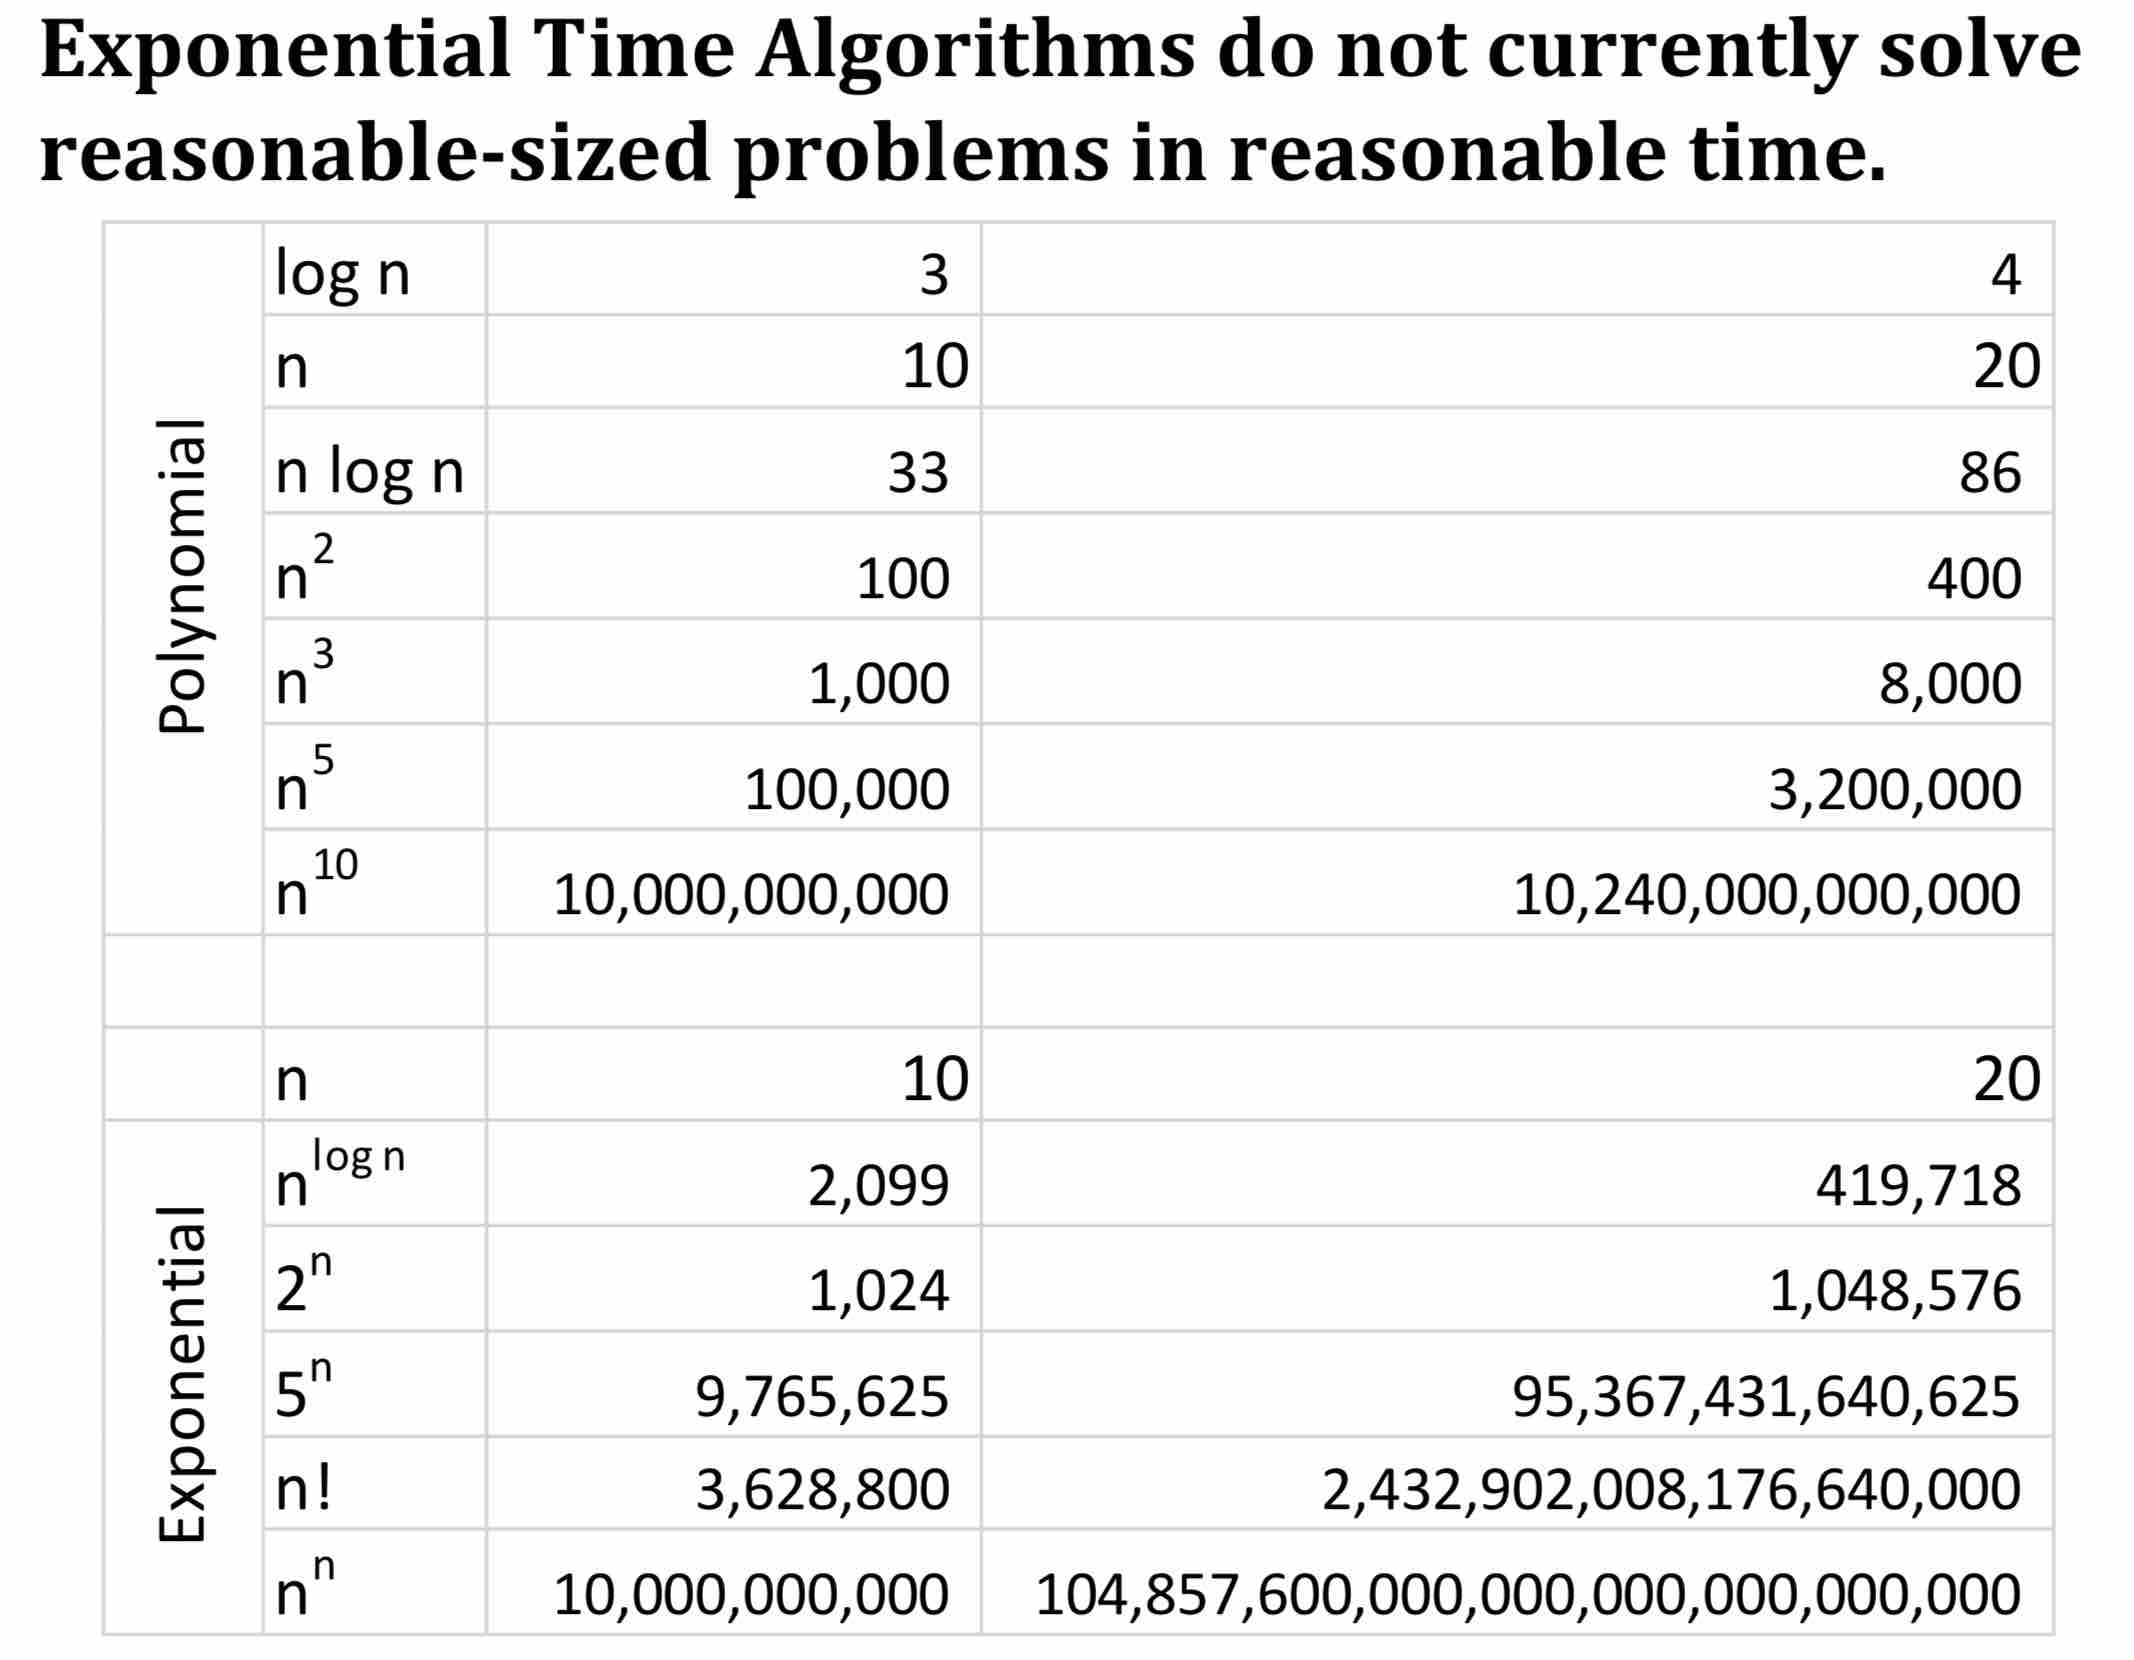
\includegraphics[scale = 0.3]{time-of-algorithms}

\section{Algorithms - Example with Bubble Sort}
The following definition comes from Merriam-Webster's dictionary.
\begin{definition}
An algorithm is a procedure for solving a mathematical problem in a finite number of steps that frequently involves repetition of an operation; broadly: a step-by-step procedure for solving a problem or accomplishing some end.
\end{definition}
\subsection{Sorting }
\url{https://en.wikipedia.org/wiki/Bubble_sort}



Bubble sort algorithm:.....


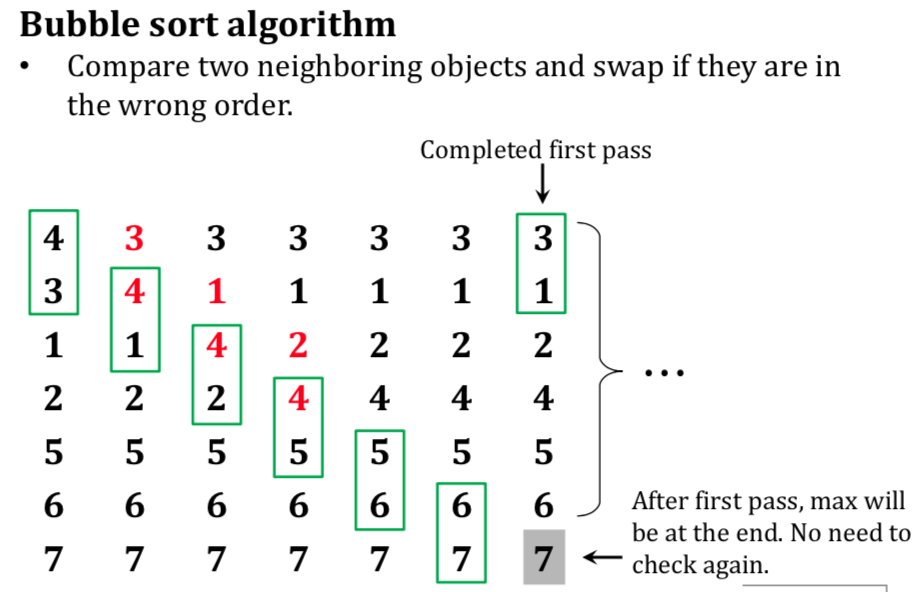
\includegraphics[scale = 0.35]{bubble-sort-alg}

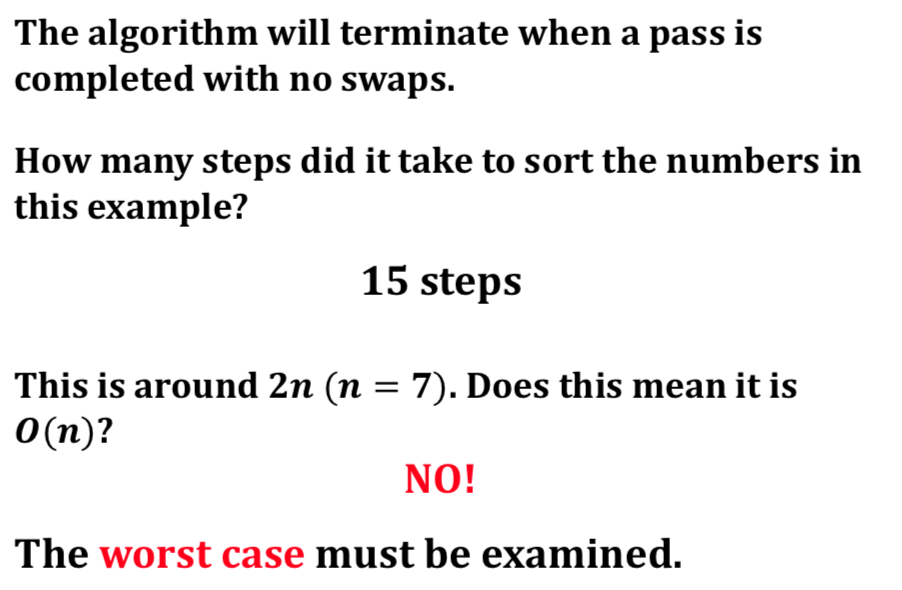
\includegraphics[scale = 0.35]{bubble-sort-complexity-1}

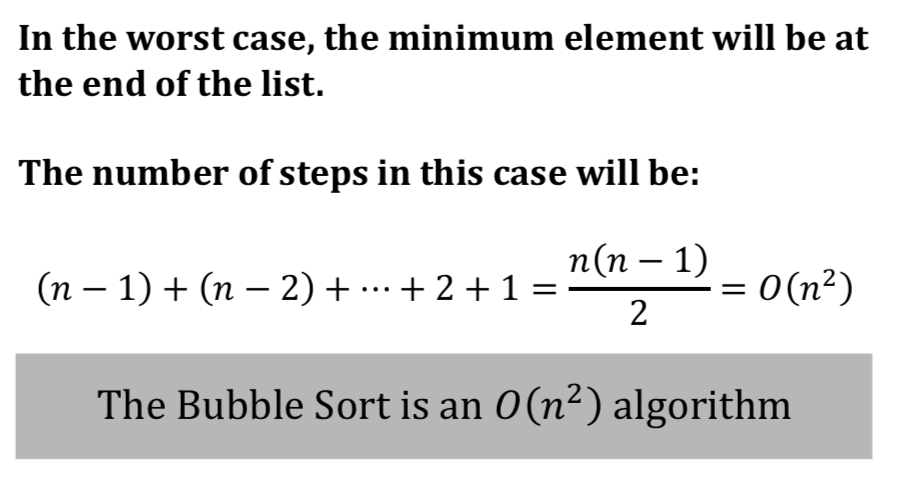
\includegraphics[scale = 0.35]{bubble-sort-complexity-2}

We can also consider the best case and average case complexity:

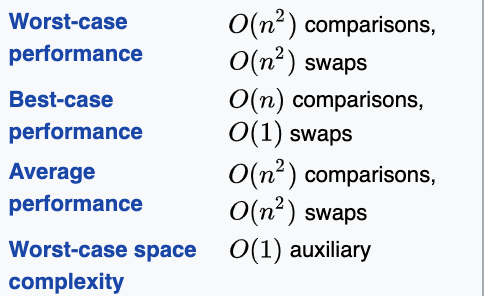
\includegraphics[scale = 0.5]{bubble-sort-complexity-wikipedia}

These can be verified experimentally  as seen in the following plot.  The random case grows quadratically just as the worst case does.  

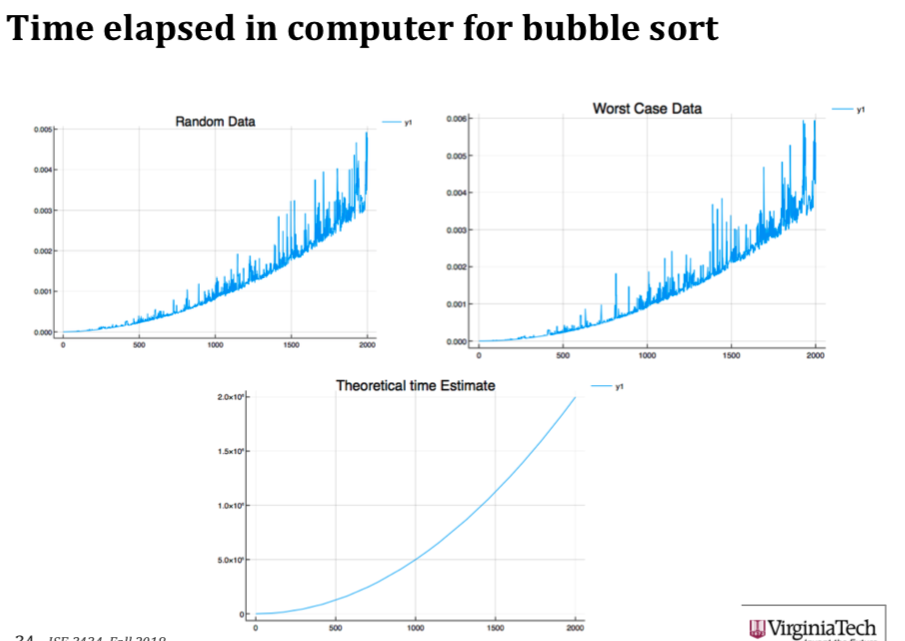
\includegraphics[scale = 0.35]{bubble-sort-computational-example}


\section{Complexity Classes}
In this subsection we will discuss the complexity classes P, NP, NP-Complete, and NP-Hard.  These classes help measure how difficult a problem is.  \textbf{Informally,} these classes can be thought of as 
\begin{itemize}
\item P - the class of efficiently solvable problems
\item NP - the class of efficiently checkable problems
\item NP-Hard - the class of problems that can solve any problem in NP
\item NP-Complete - the class of problems that are in both NP and are NP-Hard.
\end{itemize}
It is not known if $P$ is the same as NP, but it is conjectured that these are very different classes.  This would mean that the NP-Hard problems (and NP-Complete problems) are necessarily much more difficult than the problems in P.
\begin{figure}[H]
\begin{center}
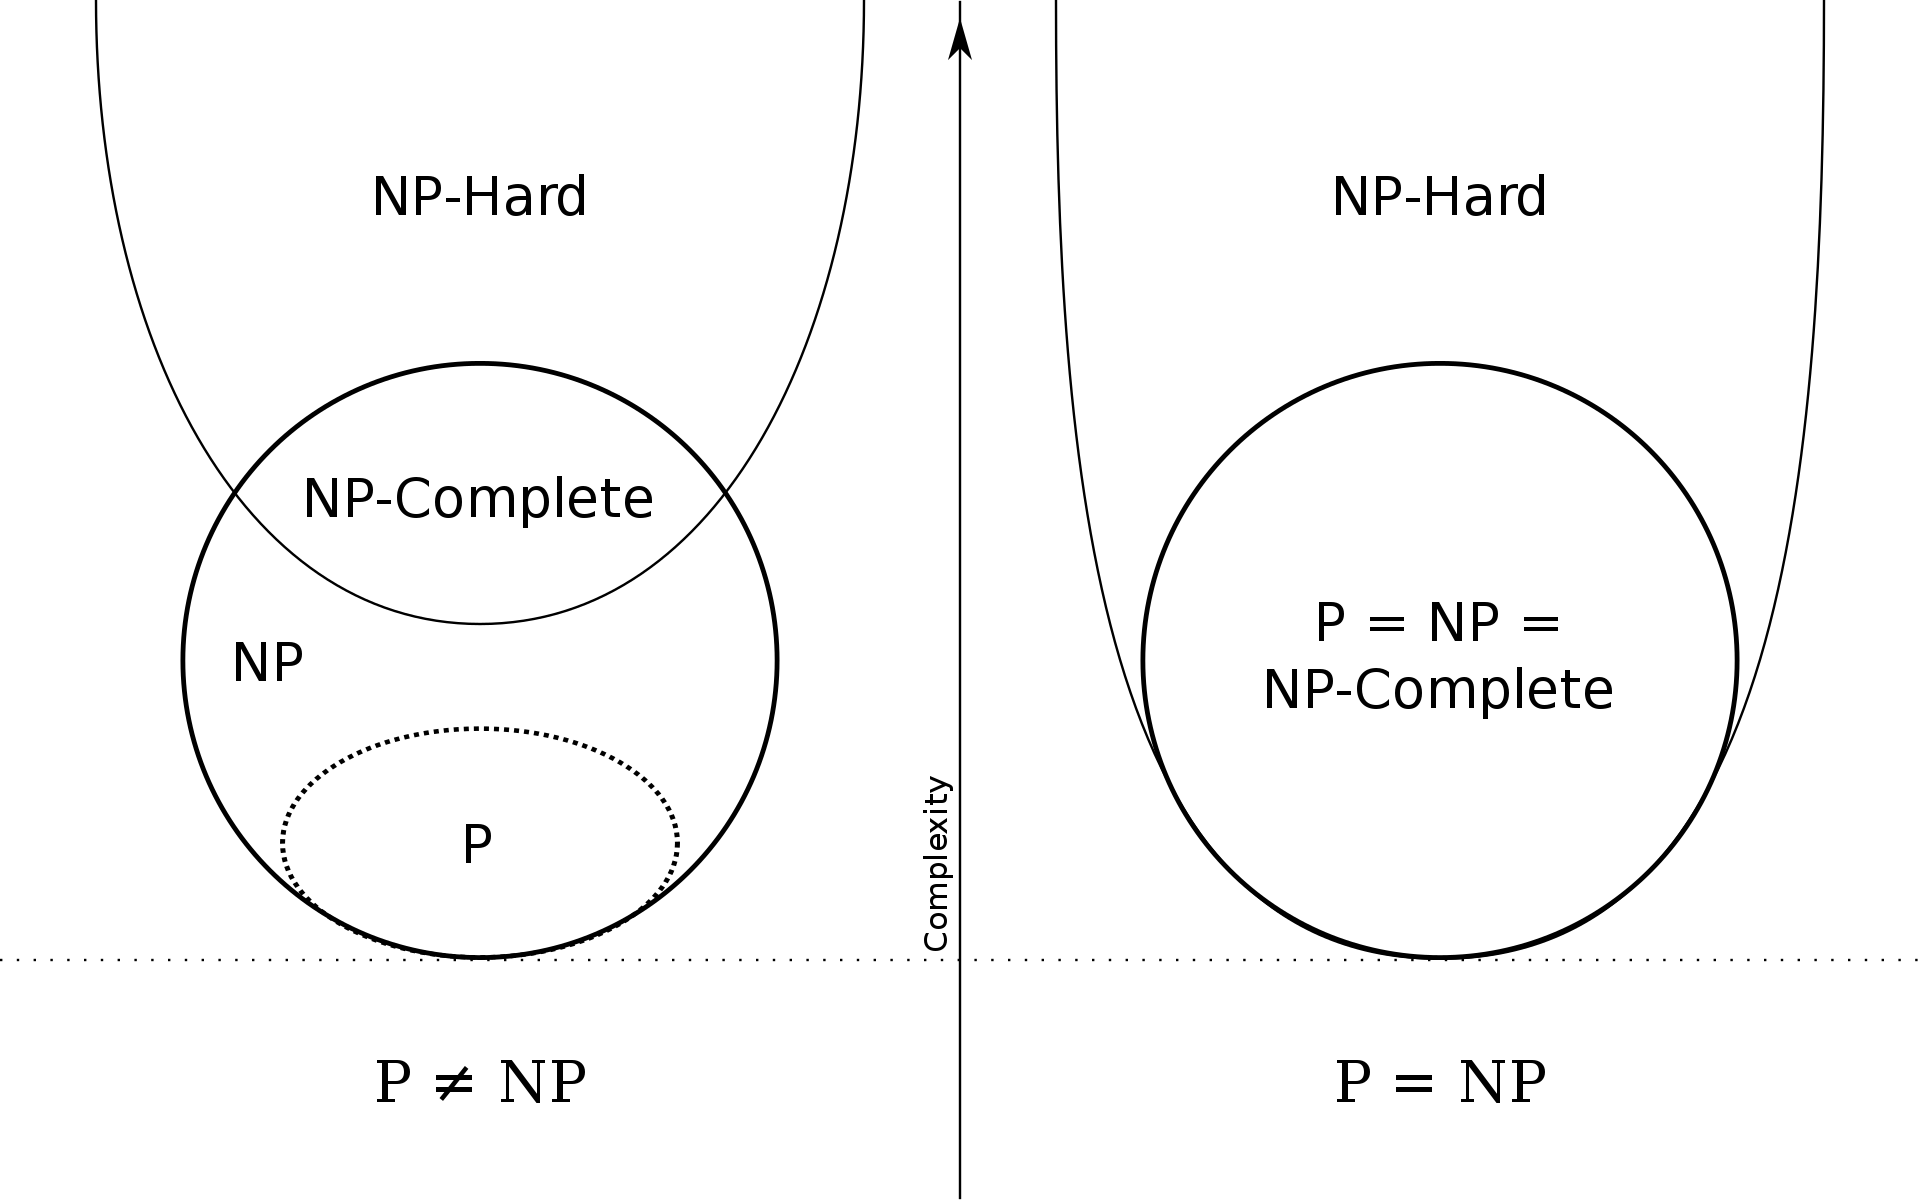
\includegraphics[scale = 0.1]{complexity-classes} \footnotemark

\end{center}
\label{fig:complexity-classes}
\caption{Complexity class possibilities.  Most academics agree that the case $P \neq NP$ is more likely.}
\end{figure}
\footnotetext{Figure from \url{https://en.wikipedia.org/wiki/NP_(complexity)}}

We will now discuss these classes more formally.
\subsection{P}
P is the class of polynomially solvable problems.  P contains tall problems for which there exists an algorithm that solves the problem in a run time bounded by a polynomial. That is, $O(n^c)$ for some constant $c$.
\begin{example}
The minimum size spanning tree problem is in P.  It can be solved, for instance, by Prim's algorithm, which  by runs in time $O(m \log n)$, where $m$ is the number of edges in the graph and $n$ is the number of nodes in the graph.  
\end{example}
\begin{example}
Linear programming is in P.  It can be solved by interior point methods in $O(n^{3.5} \phi)$ where $\phi$ represents the number of binary bits that are required to encode the problem.  These bits describe the matrix $A$, and vectors $c$ and $b$ that define the linear program.
\end{example}
\subsection{NP}
NP is the class of nondeterministic polynomial problems.  NP contains all problems in which membership can be verified in polynomial time from a certificate.

Thus, to show that a problem is in NP, you must do the following:
\begin{enumerate}
\item Describe a format for a certificate to the problem.
\item Show that given such a certificate, it is easy to verify the solution to the problem.
\end{enumerate}
\begin{example}
Integer Linear Programming is in NP.  More explicitly, the feasibility question of
\begin{center}
"Does there exists an integer vector $x$ that satisfies $Ax\leq b$"
\end{center}
is in NP.  

Although it turns out to be difficult to find such an $x$ or even prove that one exists, this problem is in NP for the following reason:  if you are given a particular $x$ and someone claims to you that it is a feasible solution to the problem, then you can easily check if they are correct.  
In this case, the vector $x$ that you were given is called a \emph{certificate}.

Note that it is easy to verify if $x$ is a solution to the problem because you just have to 
\begin{enumerate}
\item Check if $x$ is integer.
\item Use matrix multiplication to check if $Ax \leq b$ holds.
\end{enumerate}
\end{example}
\subsection{NP-Hard}
The class of problems that are called \emph{NP-Hard} are those that can be used to solve any other problem in the NP class.  
That is, problem A is NP-Hard provided that for any problem B in NP there is a transformation of problem B that preserves the size of the problem, up to a polynomial factor, into a new problem that problem A can be used to solve.

Here we think of ``if problem A could be solved efficiently, then all problems in NP could be solved efficiently".

More specifically, we assume that we have an oracle for problem A that runs in polynomial time.  An oracle is an algorithm that for the problem that returns the solution of the problem in a time polynomial in the input.   This oracle can be thought of as a magic computer that gives us the answer to the problem.   
Thus, we say that problem A is NP-Complete provided that given an oracle for problem A, one can solve any other problem B in NP in polynomial time.

Note:  These problems are not necessarily in NP.

\subsection{NP-Complete}
The class of problems that are call \emph{NP-Complete} are those which are in NP and also NP-Hard.  

We know of many problems that are NP-Complete.  For example, binary integer programming feasibility is NP-Complete.  One can show that another problem is NP-complete by 
\begin{enumerate}
\item showing that it can be used to solve binary integer programming feasibility,
\item showing that the problem is in NP.
\end{enumerate}

The first problem proven to be NP-Complete is called \emph{3-SAT}~\cite{}.  3-SAT is a special case of the \emph{satisfiability problem}.   In a satisfiability problem, we have variables $X_1, \dots, X_n$ and we want to assign them values as either \true or \false.  The problem is described with \emph{AND} operations, denoted as $\land$,  with \emph{OR} operations, denoted as $\lor$, and with \emph{NOT} operations, denoted as $\neg$.  The \emph{AND} operation $X_1 \land X_2$ returns $\true$ if BOTH $X_1$ and $X_2$ are true.  The \emph{OR} operation $X_1 \lor X_2$ returns $\true$ if AT LEAST ONE OF  $X_1$ and $X_2$ are true.  Lastly, the \emph{NOT} operation $\neg X_1$ returns there opposite of the value of $X_1$.

These can be described in the following table
\begin{align}
\true \land \true = \true\\
\true \land \false = \false\\
\false \land \false = \false\\
\false \land \true = \false
\end{align}

\begin{align}
\true \lor \true = \true\\
\true \lor \false = \true\\
\false \lor \false = \false\\
\false \lor \true = \true
\end{align}

\begin{align}
\neg \true = \false\\
\neg \false = \true
\end{align}

For example, \textbf{Missing code here}
%$$
%\neg \true \lor \false \lor \true = \true \ \ \ \ \true \and \neg \true = \false
%$$
A \emph{logical expression} is a sequence of logical operations on variables $X_1, \dots, X_n$, such that 
\begin{equation}
(X_1 \land \neg X_2 \lor X_3) \land (X_1 \lor \neg X_3) \lor (X_1 \land X_2 \land X_3).
\end{equation}

A \emph{clause} is a logical expression that only contains the operations $\lor$ and $\neg$ and is not nested (with parentheses), such as 
\begin{equation}
X_1 \lor \neg X_2 \lor X_3 \lor \neg X_4.
\end{equation}

A fundamental result about logical expressions is that they can always be reduced to a sequence of clauses that are joined by $\land$ operations, such as 
\begin{equation}
(X_1 \lor \neg X_2 \lor X_3 \lor \neg X_4) \land (X_1 \lor X_2 \lor X_3) \land (X_2 \lor \neg X_3 \lor \neg X_4 \lor X_5).
\end{equation}
The satisfiability problem takes as input a logical expression in this format and asks if there is an assignment of \true  or \false to each variable $X_i$ that makes the expression \true.  The 3-SAT problem is a special case where the clauses have only three variables in them.
 
\begin{general}{3-SAT}{\npcomplete}
Given a logical expression in $n$ variables where each clause has only 3 variables, decide if there is an assignment to the variables that makes the expression \true.
\end{general}


\begin{general}{Binary Integer Programming}{\npcomplete}
Binary Integer Programming can easily be shown to be in NP, since verifying solutions to BIP can be done by checking a linear system of inequalities.  

Furthermore, it can be shown to be NP-Complete since it can be used to solve 3-SAT.  That is, given an oracle for BIP, since 3-SAT can be modeled as a BIP,  the 3-SAT could be solved in oracle-polynomial time.
\end{general}

\section{Relevant Terminology}
We will discuss the following concepts:
\begin{itemize}
\item Feasible solutions
\item Optimal solutions
\item Approximate solutions
\item Heuristics
\item Exact Algorithms
\item Approximation Algorithms
\item Complexity class relations
\end{itemize}


\section{Matching Problem}




\begin{definition}
Given a graph $G = (V,E)$, a \emph{matching} is a subset $E' \subseteq E$ such that no vertex $v \in V$ is contained in more than one edge in $E'$.  \\
A \emph{perfect matching} is a matching were every vertex is connected to an edges in $E'$.\\
A \emph{maximal matching} is a matching $E'$ such that there is no matching $E''$ that strictly contains it.
\end{definition}


\begin{figure}[H]
\begin{center}
\includegraphics[scale = 0.5]{matchings}\footnotemark
\end{center}
\label{fig:matching}
\caption{Two possible matchings.  On the left, we have a perfect matchings (all nodes are matched).  On the right, a feasible matching, but not a perfect matching since not all nodes are matched.}

\end{figure}

\footnotetext{Figure from \url{http://www.suhendry.net/blog/?p=1647}.}






\begin{definition}{Maximum Weight Matching}
Given a graph $G = (V,E)$, with associated weights $w_e\geq 0$ for all $e \in E$, a \emph{maximum weight matching} is a matching that maximizes the sum of the weights in the matching.
\end{definition}

\begin{figure}[H]
\begin{center}
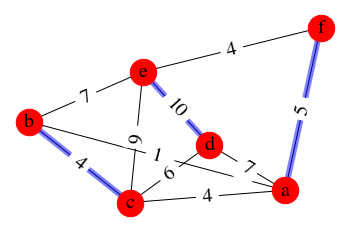
\includegraphics[scale = 0.5]{graph-for-matching-maximal}
\end{center}
\end{figure}




%
%\begin{enumerate}
%\item Feasible solution
%\item Greedy Procedure
%\end{enumerate}
%
%\begin{enumerate}
%\item Procedure
%\item Algorithm
%\begin{enumerate}
%\item Heuristic
%\item Approximation
%\item Exact
%\end{enumerate}
%\end{enumerate}
\subsection{Greedy Algorithm for Maximal Matching}
The greedy algorithm iteratively adds the edge with largest weight that is feasible to add.  
\begin{general}{Greedy Algorithm for Maximal Matching}{Complexity: $O(|E|\log(|V|))$}
\label{alg:greedy-matching}
\begin{enumerate}
\item Begin with an empty graph $(M = \emptyset)$
\item Label the edges in the graph such that $w(e_1) \geq w(e_2) \geq \dots \geq w(e_m)$
\item For $i=1, \dots, m$\\
\indent  If $M \cup\{e_i\}$ is a valid matching (i.e., no vertex is incident with two edges), then set $M \leftarrow M \cup \{e_i\}$ (i.e., add edge $e_i$ to the graph $M$)
\item Return $M$
\end{enumerate}
\end{general}

\begin{theorem}[\cite{Avis83}]
The greedy algorithm finds a 2-approximation of the maximum weighted matching problem.  That is, $w(M_{greedy}) \geq \tfrac{1}{2} w(M^*)$.
\end{theorem}
%\begin{proof}
%Proof. Let x be the weight of the first edge ( i , j ) that is selected by GREEDY, so that x is in fact an edge of maximum weight in G. Now when (i,j) and all incident edges are deleted, at most two edges of the optimal matching may be removed. Further,thesumoftheirweightscannotexceed2x. Theothern-2ormoreedgesof the optimal matching are candidates for selection at the next iteration of GREEDY. The argument may be repeated for each of the first fniterations of GREEDYII. Since all edge weights are non-negative, the theorem is proved.
%\end{proof}


\subsection{Other algorithms to look at}
\begin{enumerate}
\item Improved  Algorithm \cite{DRAKE2003211}
\item Blossom Algorithm \url{https://en.wikipedia.org/wiki/Blossom_algorithm}
\end{enumerate}



\section{Minimum Spanning Tree}
\begin{definition}
Given a graph $G = (V,E)$, a \emph{spanning tree} connected, acyclic subgraph $T$ that contains every node in $V$.
\end{definition}

\begin{center}
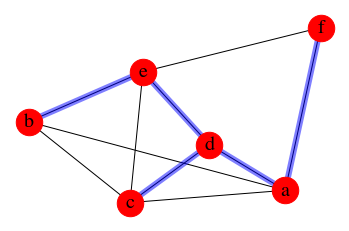
\includegraphics[scale = 0.5]{spanning-tree}
\end{center}

\begin{definition}
Given a graph $G = (V,E)$, with associated weights $w_e\geq 0$ for all $e \in E$, a \emph{maximum weight spanning tree} is a spanning tree maximizes the sum of the edge weights.
\end{definition}

\begin{center}
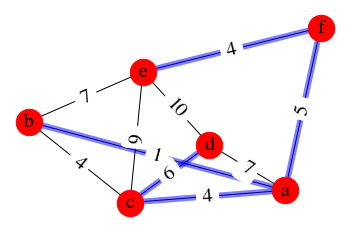
\includegraphics[scale = 0.5]{spanning-tree-MST}
\end{center}

\begin{lemma}
Let  $G$ be a  connected graph with $n$ vertices.  
\begin{enumerate}
\item $T$ is a spanning tree of $G$ if and only if $T$ has $n-1$ edges and is connected.
\item Any subgraph $S$ of $G$ with more than $n-1$ edges contains a cycle.
\end{enumerate}
\end{lemma}


See Section~\ref{sec:spanning-tree-models} for integer programming formulations of this problem.  
\subsection{Kruskal's algorithm}
\url{https://en.wikipedia.org/wiki/Kruskal\%27s_algorithm}
\begin{general}{Kruskal  - for Minimum Spanning tree}{Complexity: $O(|E| \log(|V|)$}
\label{alg:Kruskal}
\begin{enumerate}
\item Begin with an empty tree $(T = \emptyset)$
\item Label the edges in the graph such that $w(e_1) \leq w(e_2) \leq \dots \leq w(e_m)$
\item For $i=1, \dots, m$\\
\indent  If $T \cup\{e_i\}$ is acyclic, then set $T \leftarrow T \cup \{e_i\}$
\item Return $T$
\end{enumerate}
\end{general}


%\begin{general}{Acyclic Graph}{}
%\label{alg:Acyclic}
%\textbf{Input:} An acyclic graph $T$ and an edge $e$
%\textbf{Output:} Either "Yes" - $T \cup \{e\}$ contains a cycle or "No" it does not contain a cycle.
%\begin{enumerate}
%\item Begin with an empty tree $(T = \emptyset)$
%\item Label the edges in the graph such that $w(e_1) \leq w(e_2) \leq \dots \leq w(e_m)$
%\item For $i=1, \dots, m$\\
%\indent  If $T \cup\{e_i\}$ is acyclic, then set $T \leftarrow T \cup \{e_i\}$
%\item Return $T$
%\end{enumerate}
%\end{general}


%\begin{proof}
%
%\end{proof}

\subsection{Prim's Algorithm}
\url{https://en.wikipedia.org/wiki/Prim\%27s_algorithm}


\url{http://www.texample.net/tikz/examples/prims-algorithm/}


\section{Traveling Salesman Problem}
\url{https://www.youtube.com/watch?v=CPetTODX-FA}
\url{https://www.youtube.com/watch?v=R_IfyticWKQ}
\url{https://www.youtube.com/watch?v=2jncD54ryGs}

See Section~\ref{sec:tsp-models} for integer programming formulations of this problem.  Also, hill climbing algorithms for this problem such as 2-Opt, simulated annealing, and tabu search will be discussed in Section~\ref{sec:IP-Heuristics}.

\subsection{Nearest Neighbor - Construction Heuristic}
\url{https://en.wikipedia.org/wiki/Nearest_neighbour_algorithm}
Starting from any node, add the edge to the next closest node.  Continue this process.
\begin{general}{Nearest Neighbor}{Complexity: $O(n^2)$}
\label{heuristic:nearestNeighbor}
\begin{enumerate}
\item Start from any node (lets call this node 1) and label this as your current node.
\item Pick the next current node as the one that is closest to the current node that has not yet been visited.
\item Repeat step 2 until all nodes are in the tour.
\end{enumerate}
\end{general}

\subsection{Double Spanning Tree - 2-Apx}
Graphs with nice properties are often easier to handle and typically graphs found in the real world have some nice properties. The \emph{triangle inequality} comes from the idea of a triangle that the sum of the lengths of two sides always are longer than the length of the third side.  That is for side lengths $x,y,z$, we have
$$
z \leq x + y
$$
\begin{figure}[H]
\begin{center}
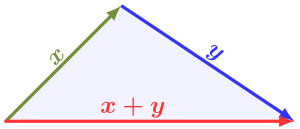
\includegraphics[scale = 0.5]{triangle-inequality}\footnotemark
\end{center}
\end{figure}
\footnotetext{Figure borrowed from \url{https://en.wikipedia.org/wiki/Triangle_inequality\#/media/File:Vector-triangle-inequality.svg }}

\begin{definition}
A complete, weighted graph $G$ (i.e., a graph that has all possible edges and a weight assigned to each edge) satisfies the \emph{triangle inequality} provided that for ever triple of vertices $a,b,c$ and edges $e_{ab}, e_{bc}, e_{ac}$, we have that 
\[
w(e_{ab}) + w(e_{bc}) \geq w(e_{ac}).
\]
\end{definition}



\begin{algorithm}
\algorithmicrequire{A graph $G = (V,E)$ that satisfies the triangle inequality}\\
\algorithmicensure{A tour that is a 2-Apx of the optimal solution}
\caption{Double Spanning Tree}\label{alg:double-spanning-tree}
\begin{algorithmic}[1]
	\State Compute a minimum spanning tree $T$ of $G$.
 	\State Double each edge in the minimum spanning tree (i.e., if edge $e_{ab}$ is in $T$, add edge $e_{ba}$. 
	\State Compute an Eulerian Tour  using these edges.
	\State Return tour that visits vertices in the order the Eulerian Tour visits them, but without repeating any vertices.
	\end{algorithmic}
\end{algorithm}

Let $S$ be the resulting tour and let $S^*$ be an optimal tour.
Since the resulting tour is feasible, it will satisfy 
\[
w(S^*) \leq w(S).
\]
But we also know that the weight of a minimum spanning tree $T$ is less than that of the optimal tour, hence
\[
w(T) \leq w(S^*).
\]
Lastly, due to the triangle inequality we know that 
\[
w(S) \leq 2 w(T),
\]
since replacing any edge in the Eulerian tour with a more direct edge only reduces the total weight.

Putting this together, we have

\[w(S) \leq 2w(T) \leq 2 w(S^*)\]
and hence, $S$ is a 2-approximation of the optimal solution.


\subsection{Christofides - Approximation Algorithm - $(3/2)$-Apx}
If we combine algorithms for minimum spanning tree and matching, we can find a better approximation algorithm.  This is given by Christofides.  Again, this is in the case where the graph satisfies the triangle inequality.  See 
\url{https://en.wikipedia.org/wiki/Christofides_algorithm} or \url{https://resources.mpi-inf.mpg.de/conferences/adfocs-15/material/Ola-Lect1.pdf} for more detail.

\end{document}